\section*{\nr.1 \titone (25 Punkte)}
\begin{enumerate}[(a)]
\item Aus 
\begin{equation}
  u(\nu)=\frac{8\pi h\nu^3}{c^3\left(\exp\left(\frac{h\nu}{k_BT}\right)-1\right)}
\end{equation}
folgt mit $\nu=\frac{c}{\lambda}$, $u(\nu)\mathrm{d}\nu=u(\lambda)\mathrm{d}\lambda$ und $\mathrm{d}\nu=-\frac{c}{\lambda^2}\mathrm{d}\lambda$, da $\mathrm{d}\lambda$ positiv sein muss
\begin{equation}
  u(\lambda)=\frac{8\pi hc}{\lambda^5\left(\exp\left(\frac{hc}{k_BT\lambda}\right)-1\right)}
\end{equation}
\item Es gilt $c=\lambda\nu$ und, nach Einstein, $\mathrm{d}c=0$, woaus folgt, dass
\begin{equation}
  0=\mathrm{d}c=\mathrm{d}(\lambda\nu)=\lambda \mathrm{d}\nu+\nu \mathrm{d}\lambda.
\end{equation}
Damit ergibt sich
\begin{equation}
  \frac{\mathrm{d}\nu}{\nu}=-\frac{\mathrm{d}\lambda}{\lambda}.
\end{equation}

Die Verläufe $u(\nu)$ und $u(\lambda)$ sind in \vref{fig:spektren1} und \vref{fig:spektren2} dargestellt, die Abhängigkeit des Spektrums vom Planckschen Wirkungsquantum findet sich in \vref{fig:spektren3}.
Aus \ref{fig:spektren3} erkennt man, dass die Wahl vom Planckschen Wirkungsquantum einen sehr signifikanten Einfluss auf das Spektrum eines schwarzen Strahlers hat. Die erforderliche Genauigkeit des Werts für $h$ ist also sehr hoch.

\begin{figure}[htbp]
\centering
% GNUPLOT: LaTeX picture with Postscript
\begingroup
  \makeatletter
  \providecommand\color[2][]{%
    \GenericError{(gnuplot) \space\space\space\@spaces}{%
      Package color not loaded in conjunction with
      terminal option `colourtext'%
    }{See the gnuplot documentation for explanation.%
    }{Either use 'blacktext' in gnuplot or load the package
      color.sty in LaTeX.}%
    \renewcommand\color[2][]{}%
  }%
  \providecommand\includegraphics[2][]{%
    \GenericError{(gnuplot) \space\space\space\@spaces}{%
      Package graphicx or graphics not loaded%
    }{See the gnuplot documentation for explanation.%
    }{The gnuplot epslatex terminal needs graphicx.sty or graphics.sty.}%
    \renewcommand\includegraphics[2][]{}%
  }%
  \providecommand\rotatebox[2]{#2}%
  \@ifundefined{ifGPcolor}{%
    \newif\ifGPcolor
    \GPcolorfalse
  }{}%
  \@ifundefined{ifGPblacktext}{%
    \newif\ifGPblacktext
    \GPblacktexttrue
  }{}%
  % define a \g@addto@macro without @ in the name:
  \let\gplgaddtomacro\g@addto@macro
  % define empty templates for all commands taking text:
  \gdef\gplbacktext{}%
  \gdef\gplfronttext{}%
  \makeatother
  \ifGPblacktext
    % no textcolor at all
    \def\colorrgb#1{}%
    \def\colorgray#1{}%
  \else
    % gray or color?
    \ifGPcolor
      \def\colorrgb#1{\color[rgb]{#1}}%
      \def\colorgray#1{\color[gray]{#1}}%
      \expandafter\def\csname LTw\endcsname{\color{white}}%
      \expandafter\def\csname LTb\endcsname{\color{black}}%
      \expandafter\def\csname LTa\endcsname{\color{black}}%
      \expandafter\def\csname LT0\endcsname{\color[rgb]{1,0,0}}%
      \expandafter\def\csname LT1\endcsname{\color[rgb]{0,1,0}}%
      \expandafter\def\csname LT2\endcsname{\color[rgb]{0,0,1}}%
      \expandafter\def\csname LT3\endcsname{\color[rgb]{1,0,1}}%
      \expandafter\def\csname LT4\endcsname{\color[rgb]{0,1,1}}%
      \expandafter\def\csname LT5\endcsname{\color[rgb]{1,1,0}}%
      \expandafter\def\csname LT6\endcsname{\color[rgb]{0,0,0}}%
      \expandafter\def\csname LT7\endcsname{\color[rgb]{1,0.3,0}}%
      \expandafter\def\csname LT8\endcsname{\color[rgb]{0.5,0.5,0.5}}%
    \else
      % gray
      \def\colorrgb#1{\color{black}}%
      \def\colorgray#1{\color[gray]{#1}}%
      \expandafter\def\csname LTw\endcsname{\color{white}}%
      \expandafter\def\csname LTb\endcsname{\color{black}}%
      \expandafter\def\csname LTa\endcsname{\color{black}}%
      \expandafter\def\csname LT0\endcsname{\color{black}}%
      \expandafter\def\csname LT1\endcsname{\color{black}}%
      \expandafter\def\csname LT2\endcsname{\color{black}}%
      \expandafter\def\csname LT3\endcsname{\color{black}}%
      \expandafter\def\csname LT4\endcsname{\color{black}}%
      \expandafter\def\csname LT5\endcsname{\color{black}}%
      \expandafter\def\csname LT6\endcsname{\color{black}}%
      \expandafter\def\csname LT7\endcsname{\color{black}}%
      \expandafter\def\csname LT8\endcsname{\color{black}}%
    \fi
  \fi
    \setlength{\unitlength}{0.0500bp}%
    \ifx\gptboxheight\undefined%
      \newlength{\gptboxheight}%
      \newlength{\gptboxwidth}%
      \newsavebox{\gptboxtext}%
    \fi%
    \setlength{\fboxrule}{0.5pt}%
    \setlength{\fboxsep}{1pt}%
\begin{picture}(7200.00,5040.00)%
    \gplgaddtomacro\gplbacktext{%
      \csname LTb\endcsname%
      \put(1342,704){\makebox(0,0)[r]{\strut{}$0$}}%
      \put(1342,1156){\makebox(0,0)[r]{\strut{}$2e-16$}}%
      \put(1342,1609){\makebox(0,0)[r]{\strut{}$4e-16$}}%
      \put(1342,2061){\makebox(0,0)[r]{\strut{}$6e-16$}}%
      \put(1342,2513){\makebox(0,0)[r]{\strut{}$8e-16$}}%
      \put(1342,2966){\makebox(0,0)[r]{\strut{}$1e-15$}}%
      \put(1342,3418){\makebox(0,0)[r]{\strut{}$1.2e-15$}}%
      \put(1342,3870){\makebox(0,0)[r]{\strut{}$1.4e-15$}}%
      \put(1342,4323){\makebox(0,0)[r]{\strut{}$1.6e-15$}}%
      \put(1342,4775){\makebox(0,0)[r]{\strut{}$1.8e-15$}}%
      \put(1474,484){\makebox(0,0){\strut{}$0$}}%
      \put(2540,484){\makebox(0,0){\strut{}$2e+14$}}%
      \put(3606,484){\makebox(0,0){\strut{}$4e+14$}}%
      \put(4671,484){\makebox(0,0){\strut{}$6e+14$}}%
      \put(5737,484){\makebox(0,0){\strut{}$8e+14$}}%
      \put(6803,484){\makebox(0,0){\strut{}$1e+15$}}%
    }%
    \gplgaddtomacro\gplfronttext{%
      \csname LTb\endcsname%
      \put(176,2739){\rotatebox{-270}{\makebox(0,0){\strut{}$u(\nu)$}}}%
      \put(4138,154){\makebox(0,0){\strut{}$\nu[Hz]$}}%
      \csname LTb\endcsname%
      \put(5816,4602){\makebox(0,0)[r]{\strut{}T=4000K}}%
      \csname LTb\endcsname%
      \put(5816,4382){\makebox(0,0)[r]{\strut{}T=5000K}}%
      \csname LTb\endcsname%
      \put(5816,4162){\makebox(0,0)[r]{\strut{}T=6000K}}%
    }%
    \gplbacktext
    \put(0,0){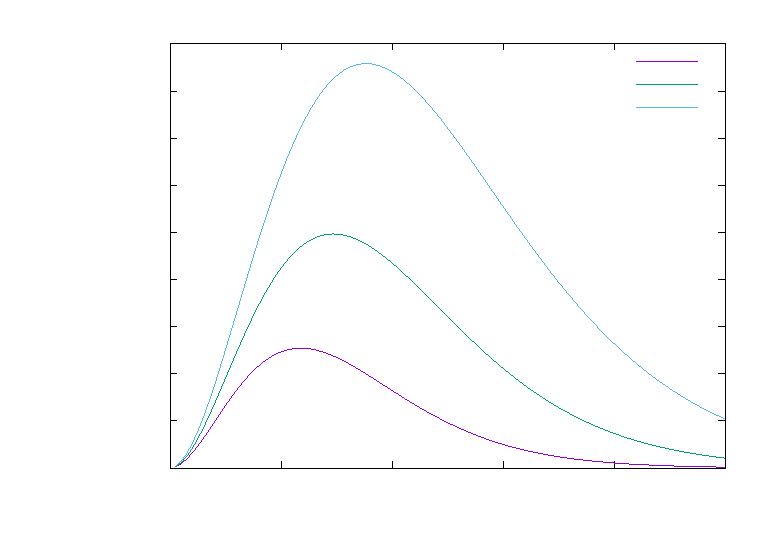
\includegraphics{spektren1}}%
    \gplfronttext
  \end{picture}%
\endgroup

\caption{Spektren von verschieden heißen schwarzen Körpern}
\label{fig:spektren1}
\end{figure}

\begin{figure}[htbp]
\centering
% GNUPLOT: LaTeX picture with Postscript
\begingroup
  \makeatletter
  \providecommand\color[2][]{%
    \GenericError{(gnuplot) \space\space\space\@spaces}{%
      Package color not loaded in conjunction with
      terminal option `colourtext'%
    }{See the gnuplot documentation for explanation.%
    }{Either use 'blacktext' in gnuplot or load the package
      color.sty in LaTeX.}%
    \renewcommand\color[2][]{}%
  }%
  \providecommand\includegraphics[2][]{%
    \GenericError{(gnuplot) \space\space\space\@spaces}{%
      Package graphicx or graphics not loaded%
    }{See the gnuplot documentation for explanation.%
    }{The gnuplot epslatex terminal needs graphicx.sty or graphics.sty.}%
    \renewcommand\includegraphics[2][]{}%
  }%
  \providecommand\rotatebox[2]{#2}%
  \@ifundefined{ifGPcolor}{%
    \newif\ifGPcolor
    \GPcolorfalse
  }{}%
  \@ifundefined{ifGPblacktext}{%
    \newif\ifGPblacktext
    \GPblacktexttrue
  }{}%
  % define a \g@addto@macro without @ in the name:
  \let\gplgaddtomacro\g@addto@macro
  % define empty templates for all commands taking text:
  \gdef\gplbacktext{}%
  \gdef\gplfronttext{}%
  \makeatother
  \ifGPblacktext
    % no textcolor at all
    \def\colorrgb#1{}%
    \def\colorgray#1{}%
  \else
    % gray or color?
    \ifGPcolor
      \def\colorrgb#1{\color[rgb]{#1}}%
      \def\colorgray#1{\color[gray]{#1}}%
      \expandafter\def\csname LTw\endcsname{\color{white}}%
      \expandafter\def\csname LTb\endcsname{\color{black}}%
      \expandafter\def\csname LTa\endcsname{\color{black}}%
      \expandafter\def\csname LT0\endcsname{\color[rgb]{1,0,0}}%
      \expandafter\def\csname LT1\endcsname{\color[rgb]{0,1,0}}%
      \expandafter\def\csname LT2\endcsname{\color[rgb]{0,0,1}}%
      \expandafter\def\csname LT3\endcsname{\color[rgb]{1,0,1}}%
      \expandafter\def\csname LT4\endcsname{\color[rgb]{0,1,1}}%
      \expandafter\def\csname LT5\endcsname{\color[rgb]{1,1,0}}%
      \expandafter\def\csname LT6\endcsname{\color[rgb]{0,0,0}}%
      \expandafter\def\csname LT7\endcsname{\color[rgb]{1,0.3,0}}%
      \expandafter\def\csname LT8\endcsname{\color[rgb]{0.5,0.5,0.5}}%
    \else
      % gray
      \def\colorrgb#1{\color{black}}%
      \def\colorgray#1{\color[gray]{#1}}%
      \expandafter\def\csname LTw\endcsname{\color{white}}%
      \expandafter\def\csname LTb\endcsname{\color{black}}%
      \expandafter\def\csname LTa\endcsname{\color{black}}%
      \expandafter\def\csname LT0\endcsname{\color{black}}%
      \expandafter\def\csname LT1\endcsname{\color{black}}%
      \expandafter\def\csname LT2\endcsname{\color{black}}%
      \expandafter\def\csname LT3\endcsname{\color{black}}%
      \expandafter\def\csname LT4\endcsname{\color{black}}%
      \expandafter\def\csname LT5\endcsname{\color{black}}%
      \expandafter\def\csname LT6\endcsname{\color{black}}%
      \expandafter\def\csname LT7\endcsname{\color{black}}%
      \expandafter\def\csname LT8\endcsname{\color{black}}%
    \fi
  \fi
    \setlength{\unitlength}{0.0500bp}%
    \ifx\gptboxheight\undefined%
      \newlength{\gptboxheight}%
      \newlength{\gptboxwidth}%
      \newsavebox{\gptboxtext}%
    \fi%
    \setlength{\fboxrule}{0.5pt}%
    \setlength{\fboxsep}{1pt}%
\begin{picture}(7200.00,5040.00)%
    \gplgaddtomacro\gplbacktext{%
      \csname LTb\endcsname%
      \put(1342,704){\makebox(0,0)[r]{\strut{}$0$}}%
      \put(1342,1286){\makebox(0,0)[r]{\strut{}$200000$}}%
      \put(1342,1867){\makebox(0,0)[r]{\strut{}$400000$}}%
      \put(1342,2449){\makebox(0,0)[r]{\strut{}$600000$}}%
      \put(1342,3030){\makebox(0,0)[r]{\strut{}$800000$}}%
      \put(1342,3612){\makebox(0,0)[r]{\strut{}$1e+06$}}%
      \put(1342,4193){\makebox(0,0)[r]{\strut{}$1.2e+06$}}%
      \put(1342,4775){\makebox(0,0)[r]{\strut{}$1.4e+06$}}%
      \put(1474,484){\makebox(0,0){\strut{}$0$}}%
      \put(2806,484){\makebox(0,0){\strut{}$5e-07$}}%
      \put(4139,484){\makebox(0,0){\strut{}$1e-06$}}%
      \put(5471,484){\makebox(0,0){\strut{}$1.5e-06$}}%
      \put(6803,484){\makebox(0,0){\strut{}$2e-06$}}%
    }%
    \gplgaddtomacro\gplfronttext{%
      \csname LTb\endcsname%
      \put(176,2739){\rotatebox{-270}{\makebox(0,0){\strut{}$u(\lambda)$}}}%
      \put(4138,154){\makebox(0,0){\strut{}$\lambda[m]$}}%
      \csname LTb\endcsname%
      \put(5816,4602){\makebox(0,0)[r]{\strut{}T=4000K}}%
      \csname LTb\endcsname%
      \put(5816,4382){\makebox(0,0)[r]{\strut{}T=5000K}}%
      \csname LTb\endcsname%
      \put(5816,4162){\makebox(0,0)[r]{\strut{}T=6000K}}%
    }%
    \gplbacktext
    \put(0,0){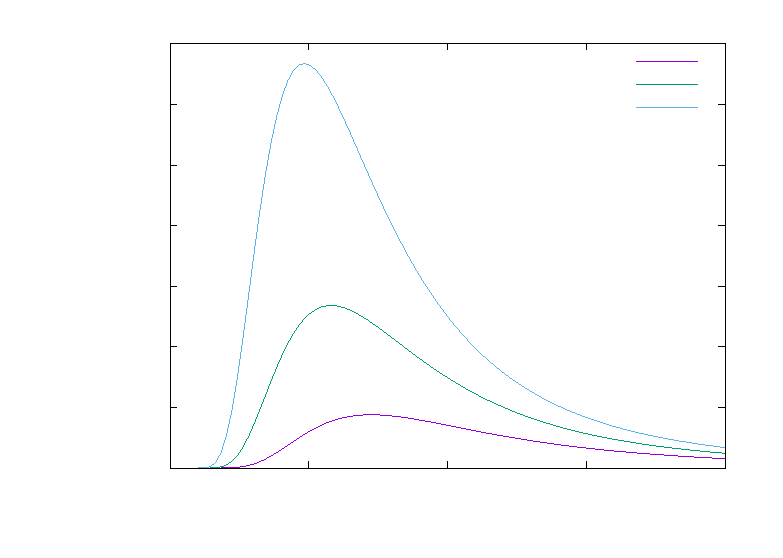
\includegraphics{spektren2}}%
    \gplfronttext
  \end{picture}%
\endgroup
 
\caption{Spektren von verschieden heißen schwarzen Körpern}
\label{fig:spektren2}
\end{figure}

\begin{figure}[htbp]
\centering
% GNUPLOT: LaTeX picture with Postscript
\begingroup
  \makeatletter
  \providecommand\color[2][]{%
    \GenericError{(gnuplot) \space\space\space\@spaces}{%
      Package color not loaded in conjunction with
      terminal option `colourtext'%
    }{See the gnuplot documentation for explanation.%
    }{Either use 'blacktext' in gnuplot or load the package
      color.sty in LaTeX.}%
    \renewcommand\color[2][]{}%
  }%
  \providecommand\includegraphics[2][]{%
    \GenericError{(gnuplot) \space\space\space\@spaces}{%
      Package graphicx or graphics not loaded%
    }{See the gnuplot documentation for explanation.%
    }{The gnuplot epslatex terminal needs graphicx.sty or graphics.sty.}%
    \renewcommand\includegraphics[2][]{}%
  }%
  \providecommand\rotatebox[2]{#2}%
  \@ifundefined{ifGPcolor}{%
    \newif\ifGPcolor
    \GPcolorfalse
  }{}%
  \@ifundefined{ifGPblacktext}{%
    \newif\ifGPblacktext
    \GPblacktexttrue
  }{}%
  % define a \g@addto@macro without @ in the name:
  \let\gplgaddtomacro\g@addto@macro
  % define empty templates for all commands taking text:
  \gdef\gplbacktext{}%
  \gdef\gplfronttext{}%
  \makeatother
  \ifGPblacktext
    % no textcolor at all
    \def\colorrgb#1{}%
    \def\colorgray#1{}%
  \else
    % gray or color?
    \ifGPcolor
      \def\colorrgb#1{\color[rgb]{#1}}%
      \def\colorgray#1{\color[gray]{#1}}%
      \expandafter\def\csname LTw\endcsname{\color{white}}%
      \expandafter\def\csname LTb\endcsname{\color{black}}%
      \expandafter\def\csname LTa\endcsname{\color{black}}%
      \expandafter\def\csname LT0\endcsname{\color[rgb]{1,0,0}}%
      \expandafter\def\csname LT1\endcsname{\color[rgb]{0,1,0}}%
      \expandafter\def\csname LT2\endcsname{\color[rgb]{0,0,1}}%
      \expandafter\def\csname LT3\endcsname{\color[rgb]{1,0,1}}%
      \expandafter\def\csname LT4\endcsname{\color[rgb]{0,1,1}}%
      \expandafter\def\csname LT5\endcsname{\color[rgb]{1,1,0}}%
      \expandafter\def\csname LT6\endcsname{\color[rgb]{0,0,0}}%
      \expandafter\def\csname LT7\endcsname{\color[rgb]{1,0.3,0}}%
      \expandafter\def\csname LT8\endcsname{\color[rgb]{0.5,0.5,0.5}}%
    \else
      % gray
      \def\colorrgb#1{\color{black}}%
      \def\colorgray#1{\color[gray]{#1}}%
      \expandafter\def\csname LTw\endcsname{\color{white}}%
      \expandafter\def\csname LTb\endcsname{\color{black}}%
      \expandafter\def\csname LTa\endcsname{\color{black}}%
      \expandafter\def\csname LT0\endcsname{\color{black}}%
      \expandafter\def\csname LT1\endcsname{\color{black}}%
      \expandafter\def\csname LT2\endcsname{\color{black}}%
      \expandafter\def\csname LT3\endcsname{\color{black}}%
      \expandafter\def\csname LT4\endcsname{\color{black}}%
      \expandafter\def\csname LT5\endcsname{\color{black}}%
      \expandafter\def\csname LT6\endcsname{\color{black}}%
      \expandafter\def\csname LT7\endcsname{\color{black}}%
      \expandafter\def\csname LT8\endcsname{\color{black}}%
    \fi
  \fi
    \setlength{\unitlength}{0.0500bp}%
    \ifx\gptboxheight\undefined%
      \newlength{\gptboxheight}%
      \newlength{\gptboxwidth}%
      \newsavebox{\gptboxtext}%
    \fi%
    \setlength{\fboxrule}{0.5pt}%
    \setlength{\fboxsep}{1pt}%
\begin{picture}(7200.00,5040.00)%
    \gplgaddtomacro\gplbacktext{%
      \csname LTb\endcsname%
      \put(1342,704){\makebox(0,0)[r]{\strut{}$0$}}%
      \put(1342,1286){\makebox(0,0)[r]{\strut{}$200000$}}%
      \put(1342,1867){\makebox(0,0)[r]{\strut{}$400000$}}%
      \put(1342,2449){\makebox(0,0)[r]{\strut{}$600000$}}%
      \put(1342,3030){\makebox(0,0)[r]{\strut{}$800000$}}%
      \put(1342,3612){\makebox(0,0)[r]{\strut{}$1e+06$}}%
      \put(1342,4193){\makebox(0,0)[r]{\strut{}$1.2e+06$}}%
      \put(1342,4775){\makebox(0,0)[r]{\strut{}$1.4e+06$}}%
      \put(1474,484){\makebox(0,0){\strut{}$0$}}%
      \put(2362,484){\makebox(0,0){\strut{}$5e-07$}}%
      \put(3250,484){\makebox(0,0){\strut{}$1e-06$}}%
      \put(4139,484){\makebox(0,0){\strut{}$1.5e-06$}}%
      \put(5027,484){\makebox(0,0){\strut{}$2e-06$}}%
      \put(5915,484){\makebox(0,0){\strut{}$2.5e-06$}}%
      \put(6803,484){\makebox(0,0){\strut{}$3e-06$}}%
    }%
    \gplgaddtomacro\gplfronttext{%
      \csname LTb\endcsname%
      \put(176,2739){\rotatebox{-270}{\makebox(0,0){\strut{}$u(\lambda)$}}}%
      \put(4138,154){\makebox(0,0){\strut{}$\lambda[m]$}}%
      \csname LTb\endcsname%
      \put(5816,4602){\makebox(0,0)[r]{\strut{}$h=6.62\cdot10^{-34}$}}%
      \csname LTb\endcsname%
      \put(5816,4382){\makebox(0,0)[r]{\strut{}$h=7\cdot10^{-34}$}}%
      \csname LTb\endcsname%
      \put(5816,4162){\makebox(0,0)[r]{\strut{}$h=8\cdot10^{-34}$}}%
      \csname LTb\endcsname%
      \put(5816,3942){\makebox(0,0)[r]{\strut{}$h=9\cdot10^{-34}$}}%
      \csname LTb\endcsname%
      \put(5816,3722){\makebox(0,0)[r]{\strut{}$h=1\cdot10^{-33}$}}%
      \csname LTb\endcsname%
      \put(5816,3502){\makebox(0,0)[r]{\strut{}$h=2\cdot10^{-33}$}}%
      \csname LTb\endcsname%
      \put(5816,3282){\makebox(0,0)[r]{\strut{}$h=3\cdot10^{-33}$}}%
      \csname LTb\endcsname%
      \put(5816,3062){\makebox(0,0)[r]{\strut{}$h=6.62\cdot10^{-33}$}}%
    }%
    \gplbacktext
    \put(0,0){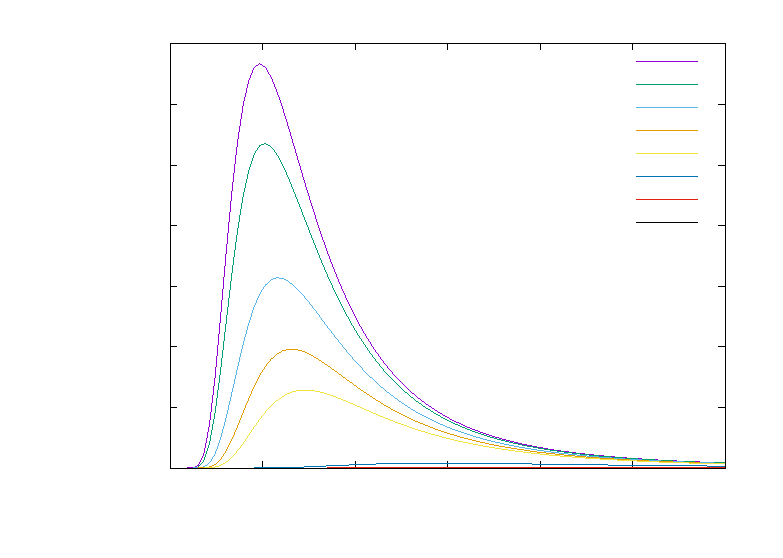
\includegraphics{spektren3}}%
    \gplfronttext
  \end{picture}%
\endgroup

\caption{Spektren für verschiedene Werte von $h$}
\label{fig:spektren3}
\end{figure}

\item Es gilt 
\begin{equation}
  \exp(x)=\sum_{n=0}^{\infty}\frac{x^n}{n!}=1+x+\frac{x^2}{2}+\dots.
\end{equation}
Für $x\to0$ folgt daraus $\exp(x)-1=x$, da die Terme höherer Ordnung vernachlässigbar werden.
Damit folgt für große $\lambda$
\begin{equation}
  \frac{8\pi hc}{\lambda^5\left(\exp\left(\frac{hc}{k_BT\lambda}\right)-1\right)}\approx\frac{8\pi hc}{\lambda^5\frac{hc}{k_BT\lambda}}=\frac{8\pi k_BT}{\lambda^4}
\end{equation}
was das Rayleigh-Jeans-Gesetz ist.


\end{enumerate}